% =====================
% Lab 2 (Adjusted version)
% =====================
\documentclass[11pt,a4paper]{book}

\usepackage[T1]{fontenc}
\usepackage[utf8]{inputenc}
\usepackage{lmodern}
\usepackage[a4paper,margin=2.5cm]{geometry}

\usepackage{amsmath,amssymb}
\usepackage{siunitx}
\sisetup{per-mode=symbol}
\usepackage{graphicx}
\usepackage{caption}
\usepackage{array}
\usepackage{hyperref}
\hypersetup{hidelinks}
\usepackage{subcaption}


% For the example table column formatting (used below)
\newcolumntype{M}[1]{>{\centering\arraybackslash}p{#1}}

\begin{document}

\chapter{Lab 2: IR spectroscopy of HCl gas}

The aim of the lab is to determine the bond length, dissociation energy, and the fundamental
frequencies/wavenumbers of a heteronuclear diatomic molecule (HCl) using its rovibrational
spectrum in the IR region. We will also determine correction terms beyond the simplest
rigid-rotor/harmonic-oscillator description in order to improve agreement with experiment.

\section{Theory}

Spectroscopy is based on the fact that electromagnetic radiation can be emitted or absorbed
when atoms, molecules, or ions undergo transitions between different energy states. These
energy changes can be associated with electronic motion (UV/Vis), vibrational motion (IR),
or rotational motion (microwave), depending on the energy scale.

In this lab, you will investigate the absorption spectrum of gaseous hydrogen chloride (HCl)
in the IR region. IR absorption increases the vibrational energy of the molecule. Because
rotational and vibrational motion are coupled, a vibrational transition is typically accompanied
by a change in rotational state, and the resulting spectrum is called a \emph{rotation--vibration
(rovibrational)} spectrum. Only molecules with a (permanent or vibration-induced) dipole moment
can give such IR spectra.

\subsection*{Rigid rotor (rotation)}
In the rigid rotor model one assumes that the molecule is completely stiff, i.e.\ the bond
length does not change during rotation. The rotational energy levels are
\begin{equation}
E_{J}=\frac{h^{2}}{8{\pi}^{2}I}J(J+1),
\label{eq:rotE}
\end{equation}
where $h=6.626\times 10^{-34}$~J\,s is Planck's constant, $J=0,1,2,\dots$ is the rotational quantum
number, and
\begin{equation}
I=\mu r^{2}
\label{eq:inertia}
\end{equation}
is the moment of inertia. Here $r$ is the bond length and $\mu$ is the reduced mass:
\begin{equation}
\mu=\frac{m_{1}m_{2}}{m_{1}+m_{2}}
\qquad \text{(diatomic molecule)}.
\end{equation}

Because experimental IR spectra are plotted versus wavenumber (cm$^{-1}$), the rotational constant
is usually expressed as a wavenumber:
\begin{equation}
\tilde{B}=\frac{h}{8{\pi}^{2}cI},
\qquad \text{(SI unit: m$^{-1}$; spectra often use cm$^{-1}$).}
\label{eq:Btilde}
\end{equation}
The rotational energy can then be written as
\begin{equation}
E_{J}=hc\tilde{B}J(J+1).
\end{equation}
Note that the energy separation between rotational levels increases with $J$ since the term is
proportional to $J(J+1)$ (Eq.~\ref{eq:rotE}); the corresponding allowed rotational transitions are shown in
Fig.~\ref{fig:ir1}.

\begin{figure}[h!]
\centering
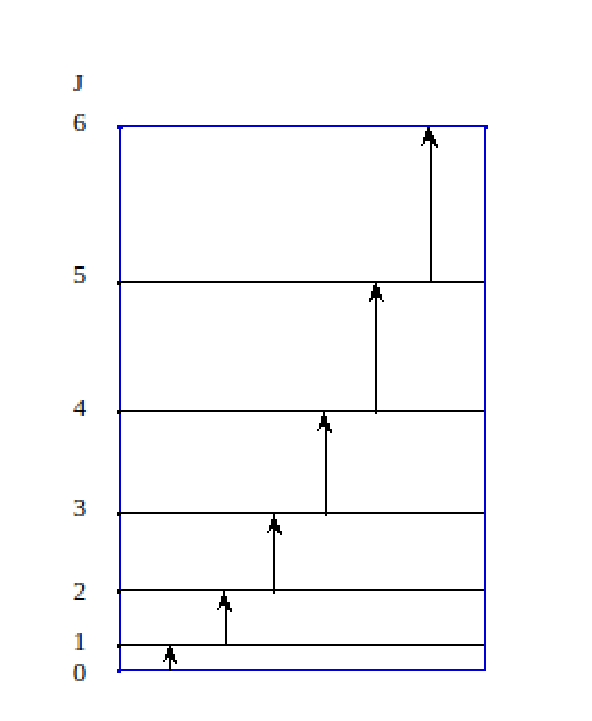
\includegraphics[scale=0.7]{ir1.eps}
\caption{Allowed rotational transitions for a rigid diatomic molecule.}
\label{fig:ir1}
\end{figure}

\subsection*{Harmonic oscillator (vibration)}
The simplest model for vibrational motion is the harmonic oscillator (``mass on a spring'').
The potential energy is
\begin{equation}
V(x)=\frac{1}{2} k x^{2},
\label{eq:Vharm}
\end{equation}
where $x=R-R_{\mathrm e}$ is the displacement from the equilibrium bond length $R_{\mathrm e}$ and $k$
is the force constant. Solving the Schr\"odinger equation gives vibrational energies
\begin{equation}
E_{v}=\hbar\omega\left(v+\frac{1}{2}\right),
\end{equation}
where $v=0,1,2,\dots$ is the vibrational quantum number and
\begin{equation}
\omega=\sqrt{\frac{k}{\mu}}
\end{equation}
is the vibrational angular frequency. In the harmonic model, the spacing between neighboring vibrational levels is constant; the corresponding allowed
vibrational transitions are shown in Fig.~\ref{fig:ir2}.


\begin{figure}[h]
\centering
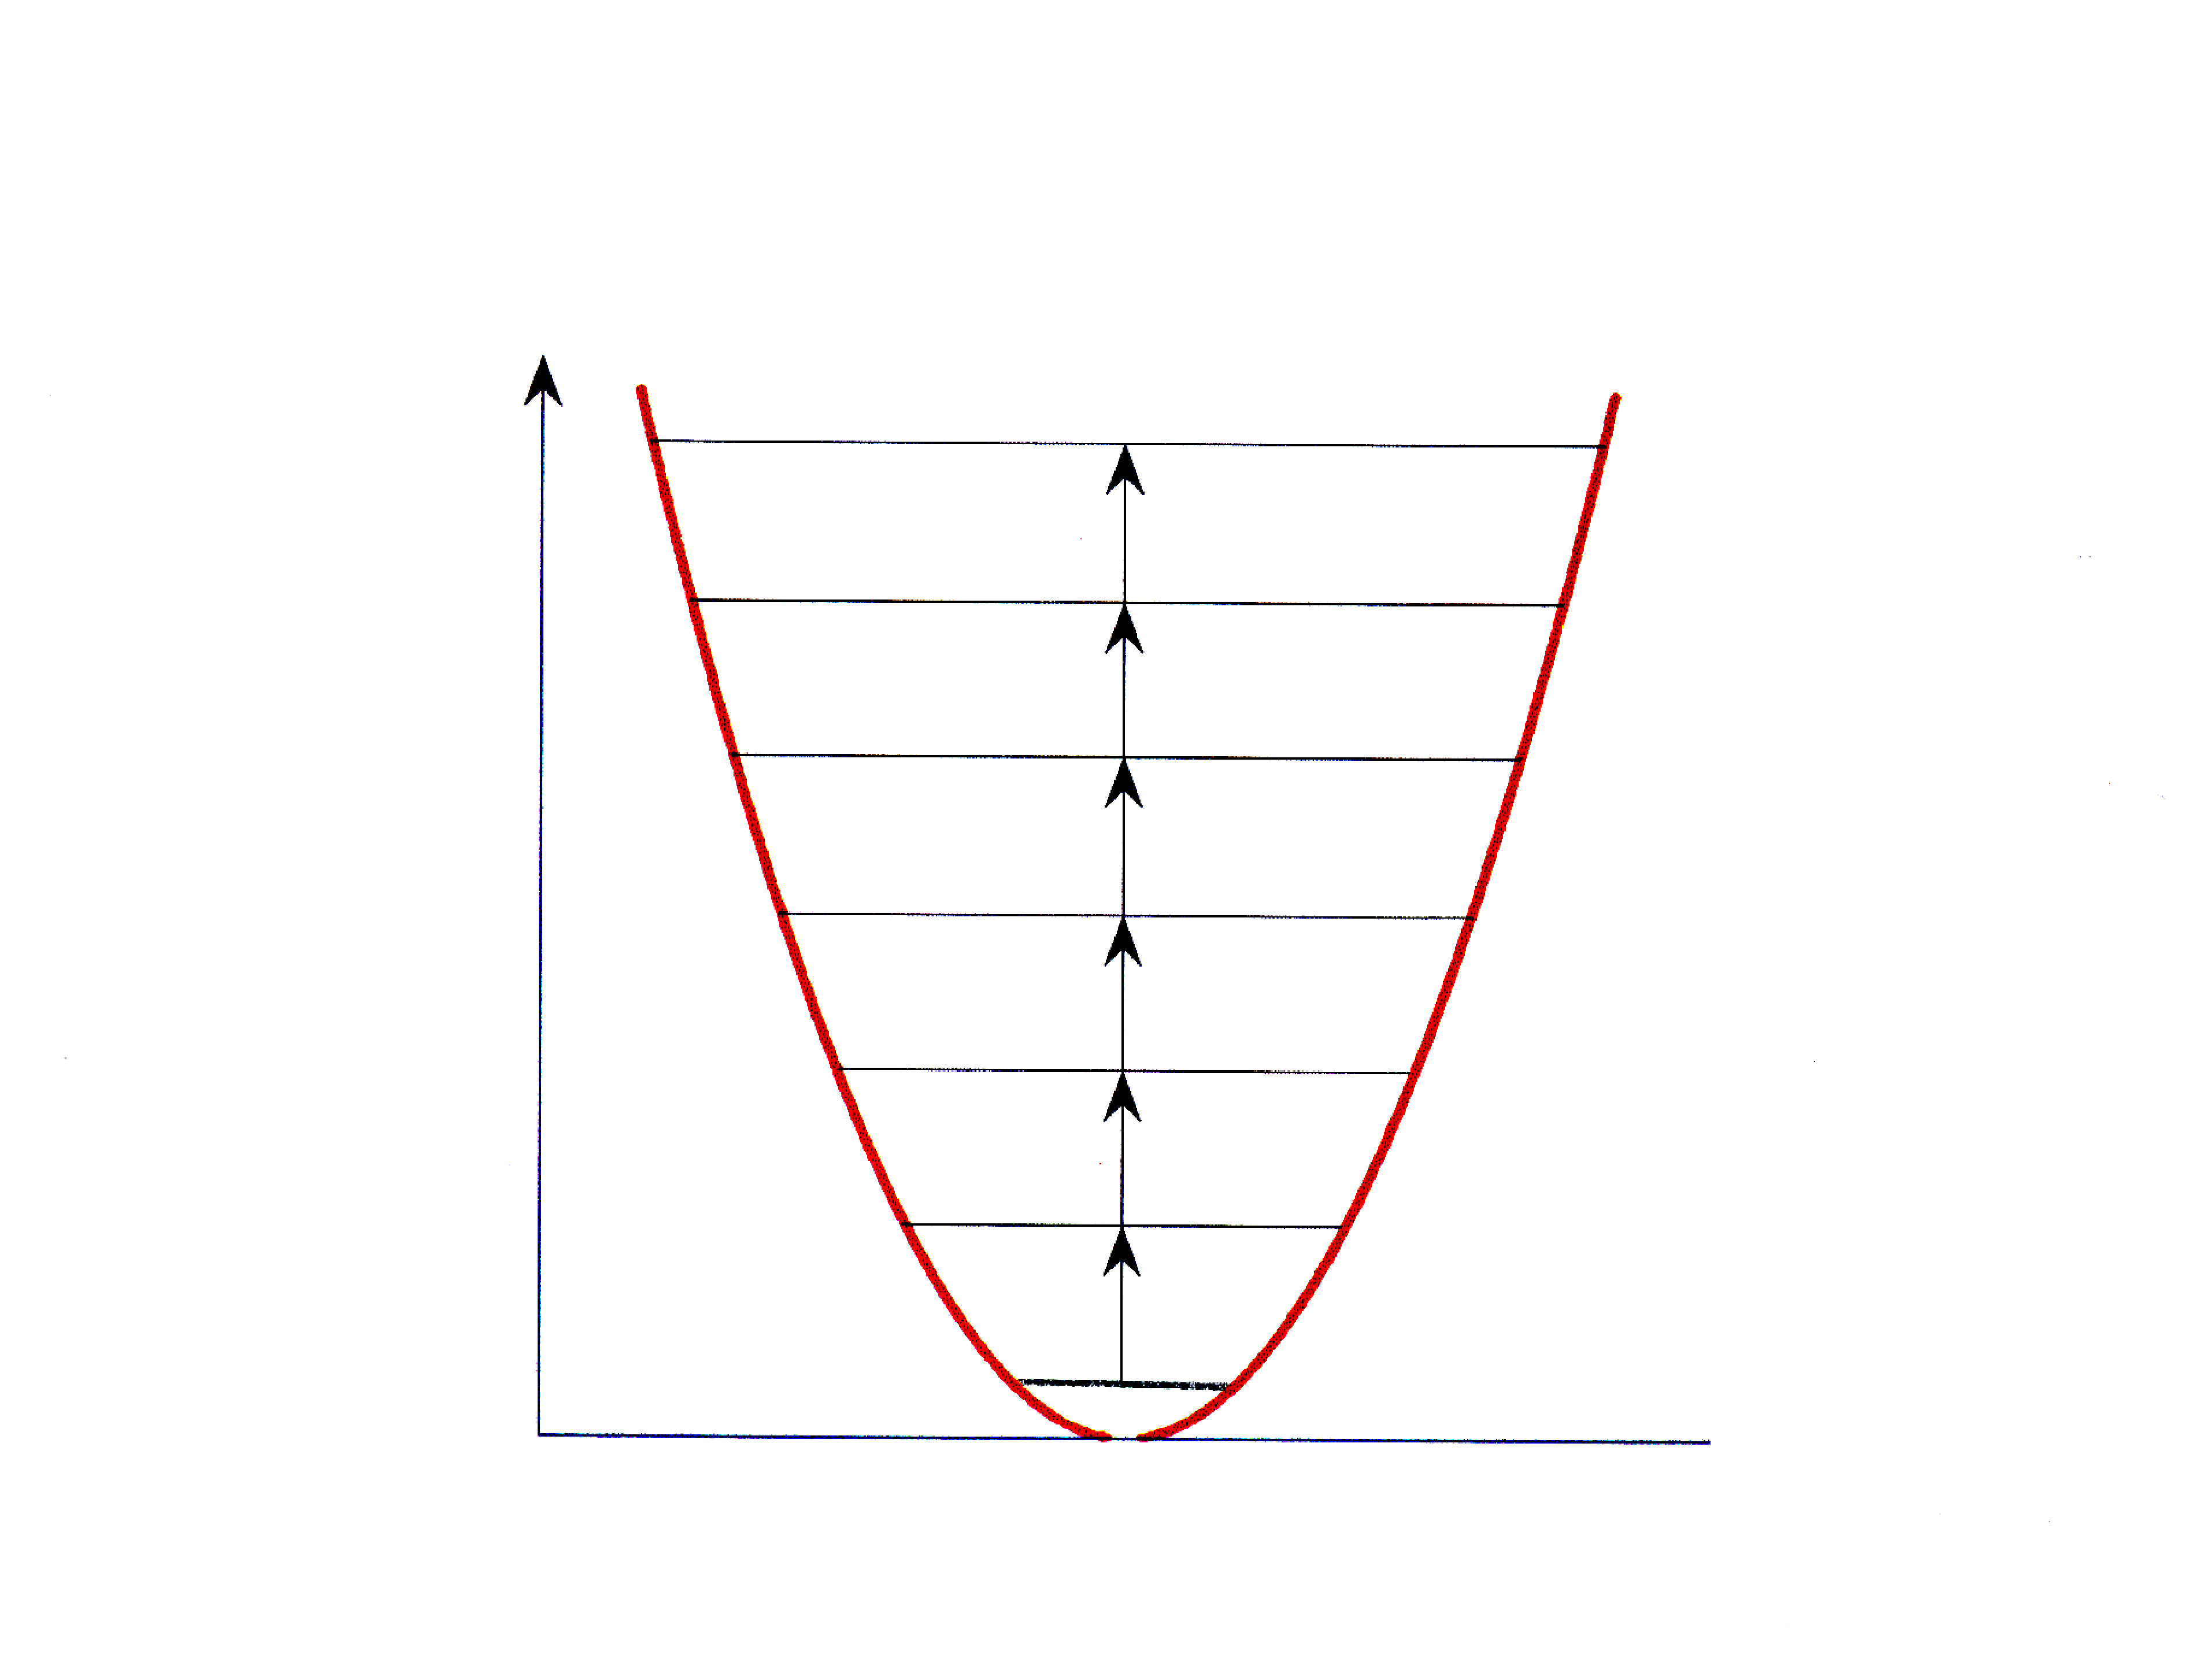
\includegraphics[scale=0.2]{ir2.eps}
\caption{Allowed vibrational transitions for a harmonic oscillator.}
\label{fig:ir2}
\end{figure}

\subsection*{Rovibration and corrections (anharmonicity + vibration--rotation coupling)}
In practice, vibrational and rotational motion occur simultaneously. As a starting point we treat the molecule
as a harmonic oscillator (vibration) combined with a rigid rotor (rotation), so that the total energy is the sum
\begin{equation}
E_{v,J}=E_v+E_J
= \hbar\omega\left(v+\frac12\right)+hc\,\tilde{B}\,J(J+1),
\label{eq:rovib_simple}\, \qquad v,J=0,1,2...
\end{equation}


The model \eqref{eq:rovib_simple} is approximate. Two important real-molecule effects are:
\begin{itemize}
\item \textbf{Anharmonicity:} the bond is not a perfect spring. At higher $v$ the vibrational level spacing decreases,
and ultimately the bond can dissociate as shown in Fig.~\ref{fig:ir3}.
\item \textbf{Vibration--rotation coupling:} the average bond length is slightly larger in higher vibrational states,
which increases the moment of inertia $I=\mu r^2$ and therefore decreases the rotational constant.
\end{itemize}

A common first improvement beyond the harmonic-oscillator/rigid-rotor model is to (i) include the leading
anharmonic correction to the vibrational energy and (ii) allow the rotational constant to depend on the
vibrational state $v$:
\begin{equation}
E_{v,J}\approx hc\left[\tilde{\omega}_e\left(v+\frac12\right)-\tilde{\omega}_e x_e\left(v+\frac12\right)^2\right]
+hc\,\tilde{B}_v\,J(J+1),
\label{eq:rovib_corr}
\end{equation}
Here a tilde denotes a wavenumber, i.e.\ $\tilde{\omega}=\omega/(2\pi c)$ (typically reported in cm$^{-1}$),
and the subscript $e$ refers to values defined at the equilibrium geometry. $\tilde{\omega}_e$ is the harmonic
vibrational constant, $x_e$ is the (dimensionless) anharmonicity constant, and the product $\tilde{\omega}_e x_e$
sets the size of the first anharmonic correction. The decrease of the rotational constant with increasing $v$
(due to a slightly larger average bond length in higher vibrational states) is often modeled as
\begin{equation}
\tilde{B}_v=\tilde{B}_e-\alpha_e\left(v+\frac12\right),
\label{eq:Bv}
\end{equation}
where $\tilde{B}_e$ is the rotational constant at the equilibrium bond length and $\alpha_e$ (cm$^{-1}$) is the
vibration--rotation coupling constant.

Anharmonicity also implies that the potential flattens at large bond distances and the molecule can eventually
reach a continuum of dissociated states. In that picture $D_0$ (introduced later) measures the depth from the
bottom of the well to the lowest dissociation limit. The anharmonic level spacing contracts with increasing $v$,
hinting at the finite number of bound levels and the possibility of bond breaking.


\begin{figure}[h!]
\centering
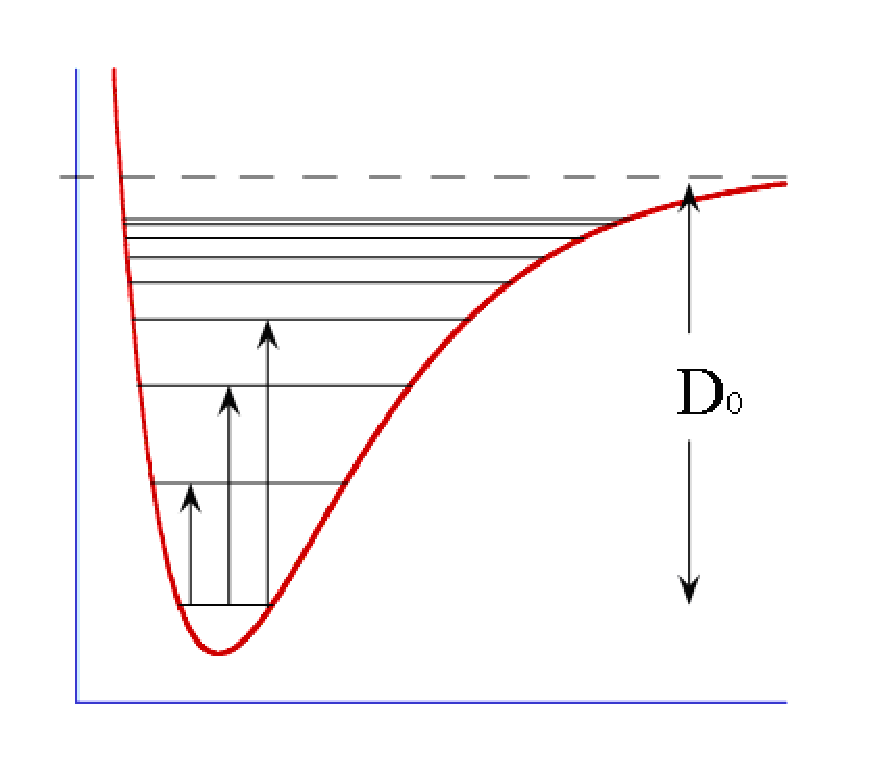
\includegraphics[scale=0.8]{ir3.eps}
\caption{Anharmonic oscillator (Morse-like). Higher $v$ states lie closer together and the bond can dissociate ($D_0$).}
\label{fig:ir3}
\end{figure}
\subsection*{Selection rules and branch structure}
For IR rovibrational spectroscopy of a heteronuclear diatomic molecule, the dominant (fundamental) band follows
\begin{equation}
\Delta v = \pm 1,
\qquad
\Delta J=\pm 1.
\end{equation}
The $\Delta J=\pm 1$ rule produces two sets (branches) of lines:
\begin{itemize}
\item \textbf{$R$ branch:} $\Delta J=+1$
\item \textbf{$P$ branch:} $\Delta J=-1$
\end{itemize}
A $Q$ branch would correspond to $\Delta J=0$, but it is not observed here in the simple diatomic rovibrational
electric-dipole picture.

In real spectra, line intensities reflect the Boltzmann population of the lower rotational levels: at room
temperature most HCl molecules occupy low $J$ values, so lines near the band origin are strongest and weaken at
higher $|m|$. Population factors and the negative $c$ coefficient (see below) together make the branch envelopes
appear smooth and gently tapered.

Anharmonicity allows overtones with
\begin{equation}
\Delta v=\pm1,\pm2,\pm3,\dots
\end{equation}
but these are much weaker than the fundamental.
\newpage
\subsection*{Line positions for the fundamental band}
We focus on the fundamental rovibrational band, i.e.\ the transition from the ground vibrational state to the first excited state
($v''=0 \rightarrow v'=1$). For this band, the observed transition wavenumbers can be written as
\begin{equation}
\tilde{\nu}_{R}=\tilde{\omega}_{0}+ (\tilde{B}_{1}+\tilde{B}_{0})(J''+1) + (\tilde{B}_{1}-\tilde{B}_{0})(J''+1)^{2}
\qquad (J''=0,1,2,\dots)
\end{equation}
for the $R$ branch ($\Delta J=+1$, with $J'=J''+1$), and
\begin{equation}
\tilde{\nu}_{P}=\tilde{\omega}_{0}- (\tilde{B}_{1}+\tilde{B}_{0})(J'+1) + (\tilde{B}_{1}-\tilde{B}_{0})(J'+1)^{2}
\qquad (J'=0,1,2,\dots)
\end{equation}
for the $P$ branch ($\Delta J=-1$, with $J''=J'+1$). Introducing $m=J''+1$ for $R$ ($m=+1,+2,\dots$) and
$m=-J'$ for $P$ ($m=-1,-2,\dots$) combines both cases into
\begin{equation}
\tilde{\nu}_{R,P}(m)=\tilde{\omega}_{0}+(\tilde{B}_{1}+\tilde{B}_{0})m+(\tilde{B}_{1}-\tilde{B}_{0})m^{2},
\label{eq:RPm}
\end{equation}
where $\tilde{B}_0 \equiv \tilde{B}_{v=0}$ and $\tilde{B}_1 \equiv \tilde{B}_{v=1}$ are the rotational constants in the lower and upper
vibrational states, respectively, and $m=\pm1,\pm2,\pm3,\dots$. Positive $m$ correspond to the $R$ branch and negative $m$ to the $P$ branch.
Because $\tilde{B}_{1}<\tilde{B}_{0}$, the coefficient $(\tilde{B}_{1}-\tilde{B}_{0})$ is negative, so the line spacing decreases slightly
as $|m|$ increases.

Only transitions that satisfy both $\Delta v=\pm1$ and $\Delta J=\pm1$ are observed here; the full set of formally
allowed transitions is narrowed by these selection rules and by dipole constraints.


\section{Preparation}
\begin{enumerate}
\item With the selection rules in mind: what molecular vibrations can be studied using IR spectroscopy? Which diatomic molecules can be studied?
\item Describe limitations of the harmonic oscillator model for IR vibrations. Describe a more realistic model introduced in this course.
\item Describe limitations of the rigid rotor model for rotation. Which more realistic correction do you know?
\item Discuss the selection rules for rotation--vibration spectroscopy and the meaning of the $P$ and $R$ branches.
\item How is the rotational constant obtained from a rovibrational spectrum?
\item Derive an expression for the bond distance $r$ as a function of the rotational constant using Eqs.~\ref{eq:inertia} and \ref{eq:Btilde}.
\end{enumerate}
\newpage
\section{Instructions}
In a full experiment, one fills a gas cuvette with HCl vapor and records an IR spectrum. \textbf{HCl is highly corrosive.}\\


\medskip
\noindent\textbf{For this lab session:} a recorded IR spectrum will be \textbf{provided} for analysis.

\subsection*{Data analysis roadmap (read this first)}
You will fit the provided line positions to Eq.~\ref{eq:RPm} by using $m$ as the x-variable.
Use the conventions:
\begin{align*}
R(J'') &: \quad m=J''+1 \qquad (J''=0,1,2,\ldots)\\
P(J'') &: \quad m=-J'' \qquad (J''=1,2,3,\ldots)
\end{align*}
Fit $\tilde{\nu}$ versus $m$ to $y=a+bx+cx^{2}$, then identify
\begin{equation}
a=\tilde{\omega}_{0},\qquad b=\tilde{B}_{1}+\tilde{B}_{0},\qquad c=\tilde{B}_{1}-\tilde{B}_{0}.
\end{equation}
Hence,
\begin{equation}
\tilde{B}_{1}=\frac{b+c}{2},\qquad \tilde{B}_{0}=\frac{b-c}{2},\qquad \alpha_{e}=\tilde{B}_{0}-\tilde{B}_{1}.
\end{equation}

\noindent\textbf{Unit note:} If you use SI values of $h$, $c$, and $\mu$ in the bond-length expression, convert
$\tilde{B}$ from cm$^{-1}$ to m$^{-1}$ via $\tilde{B}(\text{m}^{-1})=100\,\tilde{B}(\text{cm}^{-1})$.

\subsection*{Data analysis tasks}
\begin{enumerate}
\item Identify the absorption peaks for the $R$ and $P$ branches and make a table like Table~\ref{tab:ir}.
Identify as many peaks as you can.

\medskip
\noindent\textbf{Question: Why is each line within both branches split into two lines?}
\emph{Hint: consider isotopes (H$^{35}$Cl and H$^{37}$Cl) and the reduced mass.}

\begin{table}[h!]
\centering
\caption{Example table for assigned line positions (fill in your measured wavenumbers).}
\label{tab:ir}
\begin{tabular}{M{1.3cm} M{1.6cm} M{2.5cm}| M{1.3cm} M{1.6cm} M{2.5cm}}
\hline
$m$ & Peak & cm$^{-1}$ & $m$ & Peak & cm$^{-1}$\\
\hline
\hline
+10 & R(9) &  & -1  & P(1)  &  \\
+9  & R(8) &  & -2  & P(2)  &  \\
+8  & R(7) &  & -3  & P(3)  &  \\
+7  & R(6) &  & -4  & P(4)  &  \\
+6  & R(5) &  & -5  & P(5)  &  \\
+5  & R(4) &  & -6  & P(6)  &  \\
+4  & R(3) &  & -7  & P(7)  &  \\
+3  & R(2) &  & -8  & P(8)  &  \\
+2  & R(1) &  & -9  & P(9)  &  \\
+1  & R(0) &  & -10 & P(10) &  \\
\hline
\end{tabular}
\end{table}
\item Using \textit{Excel} (e.g.\ a 2nd-order polynomial trendline), \textit{Python} (e.g.\ \texttt{numpy.polyfit}),
or any other fitting tool, fit your data to
\begin{equation}
y=a+bx+cx^{2},
\label{eq:quadfit}
\end{equation}
where $x=m$ and $y=\tilde{\nu}$ (cm$^{-1}$). From this fit, $a$, $b$, and $c$ correspond to
$\tilde{\omega}_{0}$, $(\tilde{B}_{1}+\tilde{B}_{0})$, and $(\tilde{B}_{1}-\tilde{B}_{0})$, respectively.


\item From your results, calculate $\tilde{B}_{0}$ and $\tilde{B}_{1}$. Also calculate the coupling constant
\begin{equation}
\alpha_e = \tilde{B}_0 - \tilde{B}_1.
\end{equation}
From the rotational constants and Eq.~\ref{eq:Btilde}, calculate $r_{0}$ and $r_{1}$. Discuss the difference between $r_0$ and $r_1$.
What does this difference mean physically?

\item For the first overtone band, an analogous expression to Eq.~\ref{eq:RPm} leads to
\begin{equation}
\tilde{\omega}_{0}^{\prime}=2\tilde{\omega}_{e}(1-3x_{e}).
\end{equation}
We can rewrite the two relations as
\begin{equation}
\tilde{\omega}_{e}=\frac{\tilde{\omega}_{0}}{(1-2x_{e})},
\label{eq:omegae_from_omega0}
\end{equation}
and
\begin{equation}
\tilde{\omega}_{e}=\frac{\tilde{\omega_{0}}^{\prime}}{2(1-3x_{e})}.
\label{eq:omegae_from_omega0prime}
\end{equation}
Setting Eqs.~\ref{eq:omegae_from_omega0} and \ref{eq:omegae_from_omega0prime} equal gives
\begin{equation}
\frac{\tilde{\omega}_{0}}{1-2x_{e}} = \frac{\tilde{\omega}_{0}^{\prime}}{2(1-3x_{e})}.
\end{equation}
Cross-multiplying and rearranging yields
\begin{equation}
2\tilde{\omega}_{0}(1-3x_{e}) = \tilde{\omega}_{0}^{\prime}(1-2x_{e}),
\end{equation}
which can be regrouped to
\begin{equation}
\tilde{\omega}_{0}^{\prime}-2\tilde{\omega}_{0} = x_{e}(2\tilde{\omega}_{0}^{\prime}-6\tilde{\omega}_{0}).
\end{equation}
Solving for $x_e$ gives
\begin{equation}
x_{e}=\frac{\tilde{\omega_{0}}^{\prime}-2\tilde{\omega}_{0}}{2\tilde{\omega_{0}}^{\prime}-6\tilde{\omega}_{0}}.
\label{eq:xe}
\end{equation}
A literature value $\tilde{\omega_{0}}^{\prime}=5668$~cm$^{-1}$ has been reported for H$^{35}$Cl.
Using this value and your experimental $\tilde{\omega}_{0}$, calculate $x_{e}$ (Eq.~\ref{eq:xe}) and then
$\tilde{\omega}_{e}$ (Eqs.~\ref{eq:omegae_from_omega0}--\ref{eq:omegae_from_omega0prime}).

\item The dissociation energy $D_{0}$ can be estimated from
\begin{equation}
D_{0}=\frac{hc\tilde{\omega}_{e}}{4x_{e}}-\frac{1}{2}hc\tilde{\omega_{e}}\left(1-\frac{1}{2}x_{e}\right).
\end{equation}
Calculate $D_{0}$ in kJ for HCl using your result from the previous task. Compare your result with the value
given in Atkins (Table 43.1, p.\ 954).
\end{enumerate}
\clearpage
\section*{FTIR spectrum (reference)}
\begin{figure}[h!]
\centering
\includegraphics[width=\textwidth]{HCl_ftir_spectrum.png}
\caption{HCl FTIR reference spectrum.}
\end{figure}

\end{document}
